\chapter{Query Builder}
\label{chapter:QueryBuilder}

This project has another goal: to enhance the conversational search assistant to collect additional information in order to provide a query as an outcome. The query is referred to as cohort definition in the ATLAS community, as stated in section \ref{atlas}.

The following section discusses the implementation of the query builder, as well as the decisions and strategies involved.


\section{Strategy}

% explicar a estratégia de implementação do query builder
%   criação de 2 ficheiros: o cohort template e outro com as respetivas perguntas para cada field
%   pointer para o campo a ser analisado
%   divisão do query builder em 2 partes: concept set and cohort definition

So, to create a system that builds a query through a conversation with the user, the first step was to get a cohort definition generated in the ATLAS platform after implementing an experimental case.


% TODO: não sei onde meter esta figura
\begin{figure}[H]
  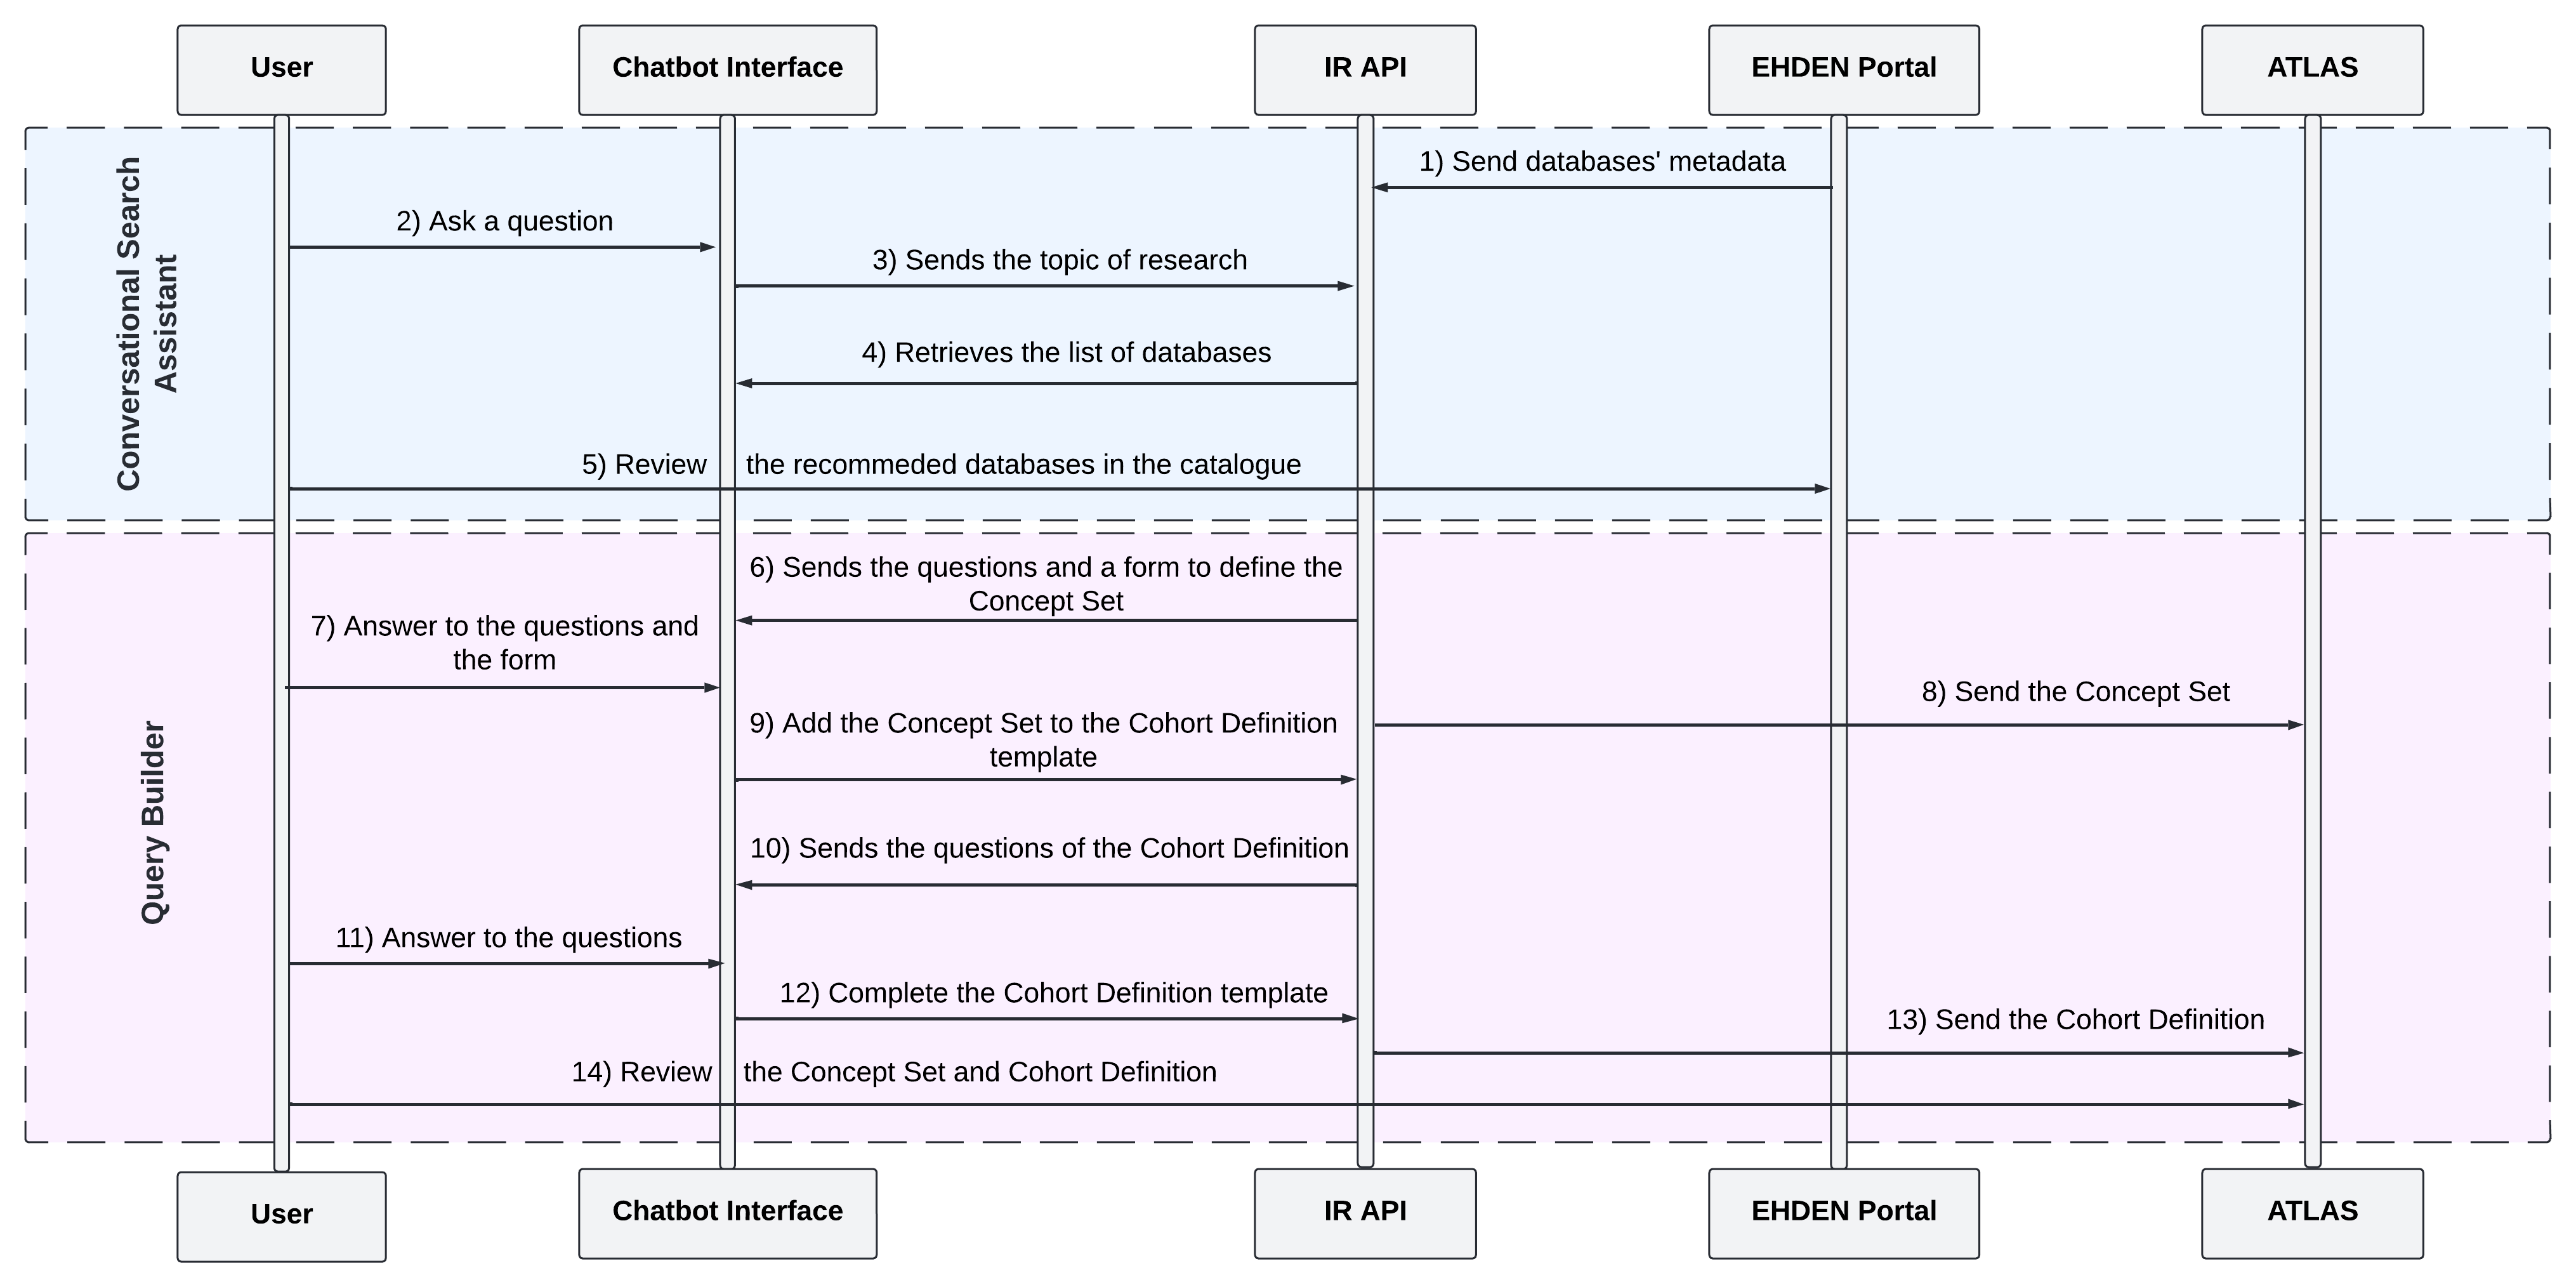
\includegraphics[width=\textwidth]{figs/chapter4/interaction_diagram.png}
  \centering
  \caption{Interaction diagram between the user, the system components and external tools.}
  \label{fig_interaction}
\end{figure}



\section{Concept Set Definiton}



\section{Cohort Definiton}



\section{ATLAS ...}





\begin{listing}[H]
\begin{minted}[breaklines]{json}
    
{
  "ConceptSets": [
    {
      "expression": {
          "items": "Do you have any other concepts to add to the concept set? (The question should be a yes with the new concepts or no response.)"
      }
    }
  ],
  "PrimaryCriteria": {
    "CriteriaList": [
      {
        "DrugExposure": {
          "CodesetId": 0,
          "First": true
        }
      }
    ],
    "ObservationWindow": {
      "PriorDays": "In terms of the observation window, what is the number of previous days? you can choose from 0, 1, 7, 14, 21, 30, 60, 90, 120, 180, 365, 548, 730 or 1095.",
      "PostDays": "In terms of the observation window, what is the number of days after? you can choose from 0, 1, 7, 14, 21, 30, 60, 90, 120, 180, 365, 548, 730 or 1095."
    },
    "PrimaryCriteriaLimit": {
      "Type": "First"
    }
  },
  "QualifiedLimit": {
    "Type": "First"
  },
  "ExpressionLimit": {
    "Type": "First"
  },
  "InclusionRules": [
    {
      "name": "has hypertension diagnosis in 1 year prior to treatment",
      "expression": {
        "Type": "ALL",
        "CriteriaList": [
          {
            "Criteria": {
              "ConditionOccurrence": {
                "CodesetId": 1
              }
            },
            "StartWindow": {
              "Start": {
                "Days": 365,
                "Coeff": -1
              },
              "End": {
                "Days": 0,
                "Coeff": 1
              },
              "UseEventEnd": false
            },
            "Occurrence": {
              "Type": 2,
              "Count": 1
            }
          }
        ],
        "DemographicCriteriaList": [],
        "Groups": []
      }
    }
  ],
  "EndStrategy": {
    "CustomEra": {
      "GapDays": 30,
      "Offset": 0
    }
  },
  "CensoringCriteria": [],
  "CollapseSettings": {
    "CollapseType": "ERA",
    "EraPad": 0
  },
  "CensorWindow": {},
  "cdmVersionRange": ">=5.0.0"
}
\end{minted}
\caption{This caption appears below the code.}
\label{lbl:questions}
\end{listing}